The classification power of the neural networks is unique for each of the decay
modes.  The performance is determined by the relative separation of the signal
and background distributions in the parameter space of the observables used as
neural network inputs.  A pathological example is the case of tau candidates
with the reconstructed decay mode of $\tau^{-} \to \pi^{-}\nu_\tau$.  If
there is no isolation activity, the neural net has no handle with which it can
separate the signal from the background.  The neural net output for
tau candidates in the testing sample (independent of the training
and validation samples) for each of the five decay mode classifications is shown
in Figure~\ref{fig:NNoutputDisributions}.

\begin{figure}[thbp]
   \setlength{\unitlength}{1mm}
   \begin{center}
      \begin{picture}(150, 195)(0,0)
         \put(0.5, 130) {\mbox{\includegraphics*[height=60mm]{tanc_chapter/figures/NNOutput_dm_0_pt_20.pdf}}}
         \put(65,  130) {\mbox{\includegraphics*[height=60mm]{tanc_chapter/figures/NNOutput_dm_1_pt_20.pdf}}}
         \put(0.5, 65) {\mbox{\includegraphics*[height=60mm]{tanc_chapter/figures/NNOutput_dm_2_pt_20.pdf}}}
         \put(65, 65) {\mbox{\includegraphics*[height=60mm]{tanc_chapter/figures/NNOutput_dm_10_pt_20.pdf}}}
         \put(33, 0) {\mbox{\includegraphics*[height=60mm]{tanc_chapter/figures/NNOutput_dm_11_pt_20.pdf}}}
      \end{picture}
   \caption[Neural network output in each decay mode]{Neural network output distributions for the
   five reconstructed tau candidate decay modes used in the TaNC for
   $Z\rightarrow\tau^{+}\tau^{-}$ events (red) and QCD dijet events (blue).  }
   \label{fig:NNoutputDisributions}
   \end{center}
\end{figure}


When a single neural network is used for classification, choosing an operating
point is relatively straightforward: the requirement on neural
network output is tuned such that the desired purity is attained.  However, in the case
of the TaNC, multiple neural networks are used.  Each network has a unique
separation power (see Figure~\ref{fig:nnPerfCurves}) and each neural network is
associated to a reconstructed decay mode that composes different relative
fractions of the signal and background tau candidates.  Therefore, a set of five
numbers is required to define an ``operating point'' (the signal efficiency and
background misidentification rate) in the TaNC output.  All points in this five
dimensional cut--space map to an absolute background fake--rate and signal
efficiency rate.  Therefore there must exist a 5D ``performance curve'' which
for any attainable signal efficiency gives the lowest fake--rate.  A direct
method to approximate the performance curve is possible using a Monte Carlo
technique.   
%
\begin{figure}[thbp]
   \setlength{\unitlength}{1mm}
   \begin{center}
     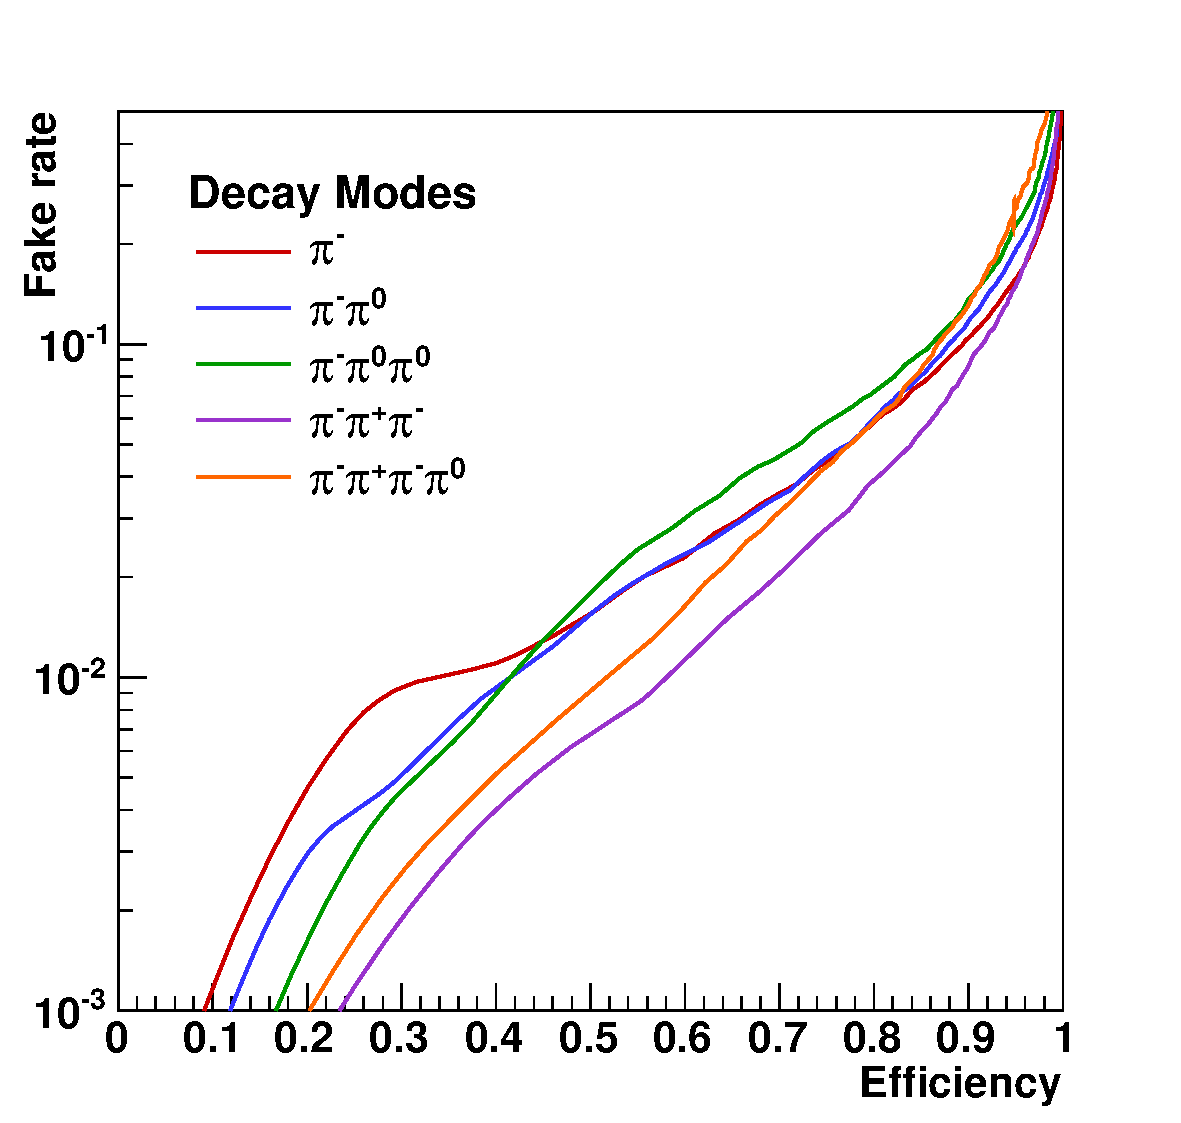
\includegraphics[width=0.98\textwidth]{tanc_chapter/figures/nnPerfCurves_20.pdf}
   \caption[Performance curves for the neural networks used in the
   TaNC]{Performance curves for the five neural networks used by the TaNC for
   tau candidates with transverse momentum greater than 20~\GeVc.  Each curve
   represents the signal efficiency (on the horizontal axis) and background
   misidentification rate (vertical axis) for a scan of the neural network
   selection requirement for a single neural network.  The efficiency (or
   misidentification rate) for each neural network performance curve is defined
   with respect to the preselected tau candidates that have the reconstructed
   decay mode associated with that neural network.  Each neural network has a
   different ability so separate signal and background as each classifier uses
   different observables as inputs.  } \label{fig:nnPerfCurves}
   \end{center}
\end{figure}

The maximal performance curve can be approximated by iteratively sampling points
in the five--dimensional cut space and selecting the highest performance points.
The collection of points in the performance curve are ordered by expected fake
rate.  During each iteration, the sample point is compared to the point before
the potential insertion position of the sample in the ordered collection.  The
sample point is inserted into the collection if it has a higher signal
identification efficiency than the point before it.  The sample point is then
compared to all points in the collection after it (\ie those with a larger fake
rate); any point with a lower signal efficiency than the sample point is
removed.  After the performance curve has been determined, the set of cuts are
evaluated on an independent validation sample to ensure that the measured
performance curve is not influenced by favorable statistical fluctuations being
selected by the Monte Carlo sampling.  The performance curves for two different
transverse momentum ranges are shown in Figure~\ref{fig:mcPerfCurves}.
%
\begin{figure}[thbp]
   \setlength{\unitlength}{1mm}
   \begin{center}
      \begin{picture}(150, 75)(0,0)
         \put(0.5, 0)
         {\mbox{\includegraphics*[width=75mm]{tanc_chapter/figures/opcurve_test_pt_5.pdf}}}
         \put(15, 60) {$\pt < 20 \GeVc$}
         \put(75, 0)
         {\mbox{\includegraphics*[width=75mm]{tanc_chapter/figures/opcurve_test_pt_20.pdf}}}
         \put(90, 60) {$20 \GeVc <\pt< 50 \GeVc$}
      \end{picture}
   \caption[Tau Neural Classifier performance curves for different \pt
   ranges]{Tau Neural Classifier performance curves for tau candidates with
   \mbox{$\pt < 20 \GeVc$} (left) and \mbox{$20 <\pt< 50 \GeVc$} (right).  The vertical
   axis represents the expected fake--rate of QCD jets and the horizontal axis
   the expected signal efficiency for hadronic tau decays.  The performance
   curve for the low transverse momentum range is worse due to leading pion
   selection.  While both true taus and QCD are removed by this cut, the
   selection preferentially keeps the QCD tau candidates with low
   multiplicities, which increases the number of QCD tau candidates passing the
   decay mode selection.  } \label{fig:mcPerfCurves}
   \end{center}
\end{figure}

The 5D performance curve can also be parameterized by using the probability for
a tau candidate to be identified for a given decay mode.  
An artificial neural network maps a point in the space of input observables to
some value of neural network output $x$.  The neural network training error is
given by Equation~\ref{eq:NNerrorFunc}.  A given point in the vector space
spanned by the neural network input observables (denoted as ``feature space'')
contributes to the neural network training error $E$ by 
\begin{equation}
   E' = (1 - x)^2\cdot\rho^\tau + x^2\cdot\rho^{QCD}
   \nonumber
\end{equation}
where $\rho^\tau (\rho^{QCD})$ denotes the training sample density of the
$\tau$ signal and QCD--jet background at that point in feature space.

The value $x$ assigned by the neural network to this region in feature space
should satisfy the requirement of minimal error:
\begin{align}
   \frac{\partial E'}{\partial x} &= 0 \nonumber \\ 
   0 &= -2(1-x)\cdot\rho^\tau+2x\cdot\rho^{QCD} \nonumber \\ 
   x &= \frac{\rho^\tau} {\rho^\tau + \rho^{QCD}} \label{eq:probFracToX} \\ 
   \rho^\tau &= x(\rho^\tau + \rho^{QCD}) \nonumber \\ 
   \frac{\rho^{QCD}}{\rho^\tau} &= \frac{1}{x} - 1  \label{eq:rawTransformX}
\end{align}
The ratio $\frac{\rho^{QCD}}{\rho^\tau}$ corresponds to the ratio of
the normalized probability density functions of signal and background input
observable distributions, \ie $\int \rho^{\tau} d\vec x = 1$.

In the case of multiple neural networks, one can derive a formula that maps the
output $x_j$ of the neural network corresponding to decay mode $j$ according to
the ``prior probabilities'' $p_j^\tau (p_j^{QCD})$ for true $\tau$ lepton
hadronic decays (quark and gluon jets) to pass the preselection criteria and
be reconstructed with decay mode $j$.
By substituting $\rho^s \rightarrow \rho^s p_j^s$ for $s \in \{\tau, QCD\}$ in
Equation~\ref{eq:probFracToX}, the output $x_j$ can be related to $p_j^\tau
(p_j^{QCD})$ by 
\begin{equation}
   x_j' = \frac{\rho^\tau \cdot p_j^\tau} 
   {\rho^\tau \cdot p_j^\tau + \rho^{QCD} \cdot p_j^{QCD} }
   = \frac{p_j^\tau} 
   {p_j^\tau + \frac{\rho^{QCD}}{\rho^\tau} \cdot p_j^{QCD} }
   \label{eq:probFracToXWithPriors}
\end{equation}
Substituting Equation~\ref{eq:rawTransformX} into
Equation~\ref{eq:probFracToXWithPriors} yields the transformation of the output
$x_j$ of the neural neural network corresponding to any selected decay mode $j$
to a single discriminator output $x_j'$ which for a given point on the optimal
performance curve should be independent of $j$.
\begin{equation}
   x_j' = \frac{p_j^\tau} 
   {p_j^\tau + \left(\frac{1}{x_j}-1\right)\cdot p_j^{QCD} }
   \label{eq:TransformCut}
\end{equation}
In this manner a single number (the ``transform cut'') given by
Equation~\ref{eq:TransformCut} can be used to specify any point on the
performance curve.  The training sample neural network output after the
transformation has been applied is shown in
Figure~\ref{fig:transformedNNOutput}.  The performance curve for the cut on the
transformed output is nearly identical to the optimal performance curve
determined by the Monte Carlo sampling technique. 

The discriminator output of the TaNC algorithm is a continuous quantity,
enabling analysis specific optimization of the selection to maximize
sensitivity.  For the convenience of the user, four operating point benchmark
selections are provided in addition to the continuous output. The four operating
points are chosen such that for tau candidates with transverse momentum between
20 and 50~\GeVc, the expected QCD dijet fake rate will be 0.1\%, 0.25\%,
0.50\% and 1.0\%, respectively.  
%
\begin{figure}[thbp]
   \setlength{\unitlength}{1mm}
   \begin{center}
      \begin{picture}(150, 75)(0,0)
         \put(0.5, 0)
         {\mbox{\includegraphics*[width=75mm]{tanc_chapter/figures/opcurve_train_pt_20_with_transform.pdf}}}
         \put(14, 60) {20 GeV/c $<\pt<$ 50 GeV/c}
         \put(75, 0)
         {\mbox{\includegraphics*[width=75mm]{tanc_chapter/figures/opcurve_test_pt_20_with_transform.pdf}}}
         \put(90, 60) {20 GeV/c $<\pt<$ 50 GeV/c}
      \end{picture}
   \caption[Tau Neural Classifier transformation performance]{Tau Neural
   Classifier performance curves for tau candidates with \mbox{$20 < \pt
   < 50 \GeVc$}.  The figure on the left compares the optimal performance curve
   determined by the Monte Carlo sampling method (red) to the performance curve
   obtained by scanning the ``transform cut'' (blue) defined in
   Equation~\ref{eq:TransformCut} from zero to one.  The figure on the right is
   the same set of cuts (and cut transformation values) applied on an
   independent sample to remove any biases introduced by the Monte Carlo
   sampling.  The four dashed lines indicate the performance for the four
   benchmark points.  } \label{fig:tancCurvesWithTransform}
   \end{center}
\end{figure}
%
\begin{figure}[thbp]
   \setlength{\unitlength}{1mm}
   \begin{center}
     \includegraphics*[width=0.6\textwidth]{tanc_chapter/figures/NNOutput_transform_5_200_preselection.pdf}
   \caption[Transformed neural network output]{Transformed TaNC neural network
   output for tau candidates with transverse momentum between 20 and 50~\GeVc
   that pass the pre--selection criteria.  The neural network output for each
   tau candidate has been transformation according to
   Equation~\ref{eq:TransformCut}.  The decay mode probabilities
   $\rho^{bkg}_i$, $\rho^{signal}_i$ are computed using the entire transverse
   momentum range of the sample.  } \label{fig:transformedNNOutput}
   \end{center}
\end{figure}
